% Polar coordinates: circles and rays, with one cell r..r+dr, theta..theta+dtheta shaded. Generated by a short script.
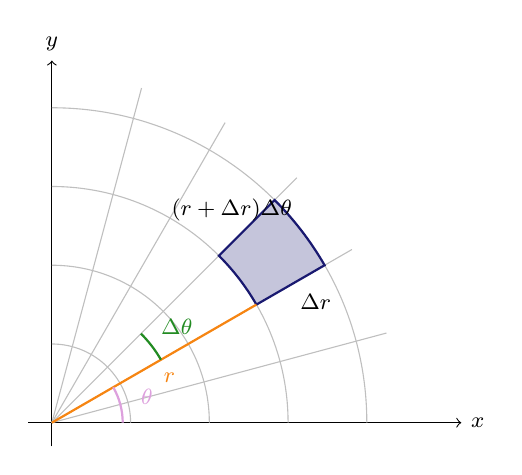
\begin{tikzpicture}[scale=1.0]
\draw[->] (-0.3,0)--(5.2,0) node[right,font=\footnotesize] {$x$};
\draw[->] (0,-0.3)--(0,4.6) node[above,font=\footnotesize] {$y$};
\draw[black!25] (1,0) arc (0:90:1);
\draw[black!25] (2,0) arc (0:90:2);
\draw[black!25] (3,0) arc (0:90:3);
\draw[black!25] (4,0) arc (0:90:4);
\draw[black!25] (0,0)--(4.250,1.139);
\draw[black!25] (0,0)--(3.811,2.200);
\draw[black!25] (0,0)--(3.111,3.111);
\draw[black!25] (0,0)--(2.200,3.811);
\draw[black!25] (0,0)--(1.139,4.250);
\fill[MidnightBlue!25,draw=MidnightBlue,thick] (30:3) arc (30:45:3) -- (45:4) arc (45:30:4) -- cycle;
\draw[BurntOrange,thick] (0,0)--(30:3);
\node[BurntOrange,font=\footnotesize,below right] at (30:1.5) {$r$};
\node[font=\footnotesize,below right] at (30:3.5) {$\Delta r$};
\node[font=\footnotesize,above left] at (37.5:4) {$(r+\Delta r)\Delta\theta$};
\draw[Plum,thick] (0.9,0) arc (0:30:0.9);
\node[Plum,font=\footnotesize] at (15.0:1.25) {$\theta$};
\draw[ForestGreen,thick] (30:1.6) arc (30:45:1.6);
\node[ForestGreen,font=\footnotesize] at (37.5:2.0) {$\Delta\theta$};
\end{tikzpicture}
